\section{Introduction}
In this chapter the project planning will be revised. More specifically the \acp{WFD} and \acp{WBS} of the midterm and final reports and the Gantt chart. These have been updated because now it is more clear as to which tasks have to be performed for the remainder of the project. Also, the work flow for the simulator has been added to the charts. In sections \ref{WFD} the revised \alc{WFD} will be shown. This is followed by section \ref{WBS}, which shows the updated \acl{WFD}. The final section gives the Gantt chart, our timeline for this project.

\section{\acl{WFD}}
\label{WFD}
The tasks to be done on the simulator have been updated and presented in more detail. Some tasks have also been 
changed in the \acp{WFD}: they now start earlier or later so as to better describe the work flow of the project. 
The tasks in the green and blue boxes respectively describe the simulator design finalization and tradeoff execution in more detail. Red boxes are tasks which are explicitly needed for the \ac{MTR}. The updated \ac{WFD} of the \ac{MTR} is given in figure \ref{fig:WFmidterm2}, page \pageref{fig:WFmidterm2}.

\begin{figure}
\centering
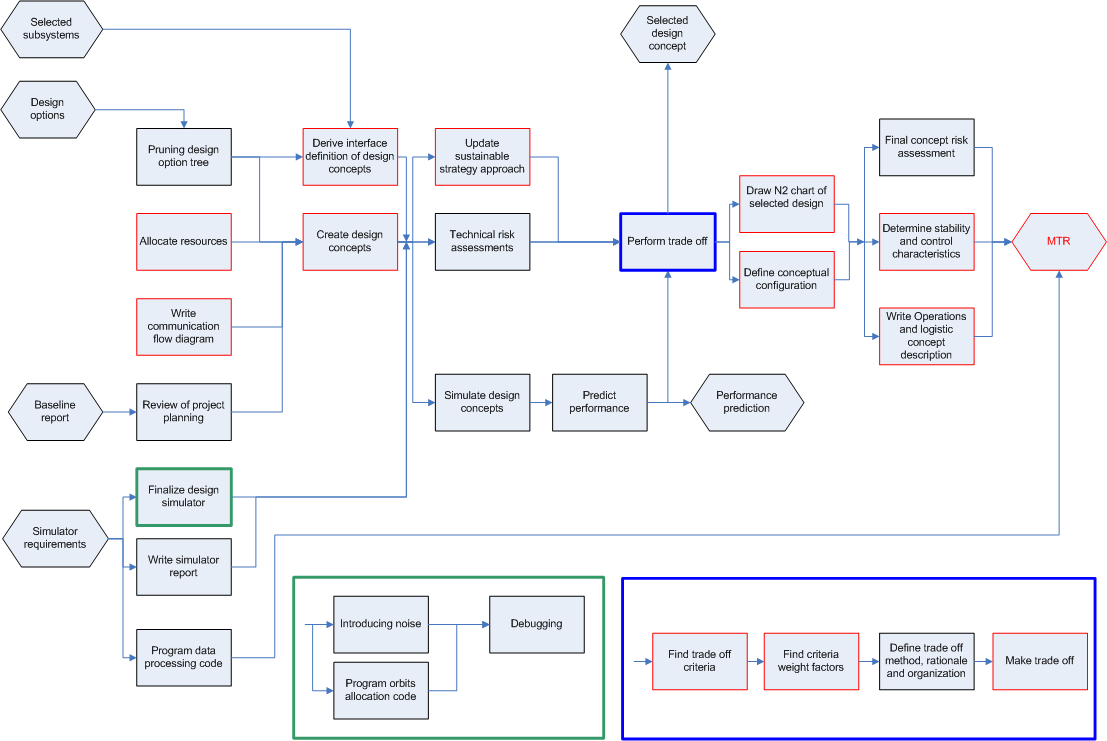
\includegraphics[width=\textheight, angle=90]{chapters/img/Workflow_diagram_MTR_v2.png}
\caption{Updated work flow diagram for the mid-term report}
\label{fig:WFmidterm2}
\end{figure}

The \acp{WFD} of the final report have also been updated. In retrospect, a very important part if the final report was not 
present in the \acp{WFD}: perfecting the design and the feasibility determination. Now these tasks have been added
to the daigram to make it complete. As with the \ac{WFD} of the \ac{MTR}, all boxes in red are explicitly required
for the final report. The diagram can be seen in figure \ref{fig:WFfinal2}, page \pageref{fig:WFfinal2}.

\begin{figure}
\centering
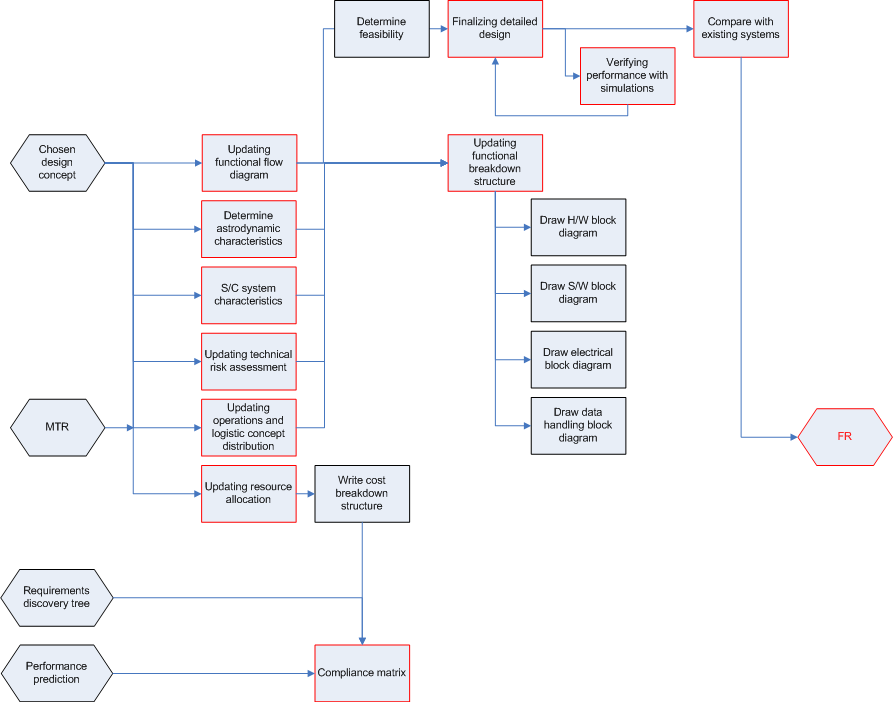
\includegraphics[width=\textheight, angle=90]{chapters/img/Workflow_diagram_FR_v2.png}
\caption{Updated work flow diagram for the final report}
\label{fig:WFfinal2}
\end{figure}


\section{\acl{WBS}}
\label{WBS}
The \acp{WBS} have been updated like the work flow diagrams. Some extra and other more detailed tasks
defined in the \acp{WFD} have also been added to these structures. Also, the layout has been changed somewhat to improve readability and correctness. The updated \acp{WBS} can be seen in figures \ref{fig:WBmidterm2} and \ref{fig:WFfinal2}, starting on page \pageref{fig:WBmidterm2}.

\begin{figure}
\centering
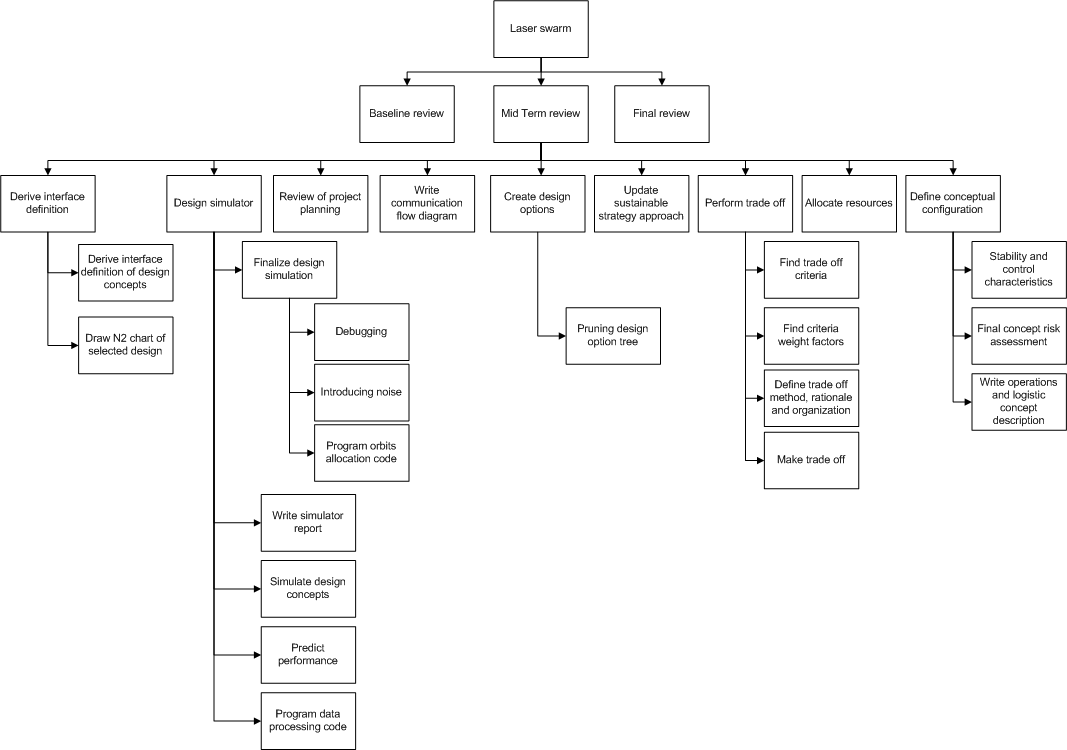
\includegraphics[width=\textheight, angle=90]{chapters/img/Workbreakdown_structure_MTR_v2.png}
\caption{Updated work break-down structure for the mid-term report}
\label{fig:WBmidterm2}
\end{figure}

\begin{figure}
\centering
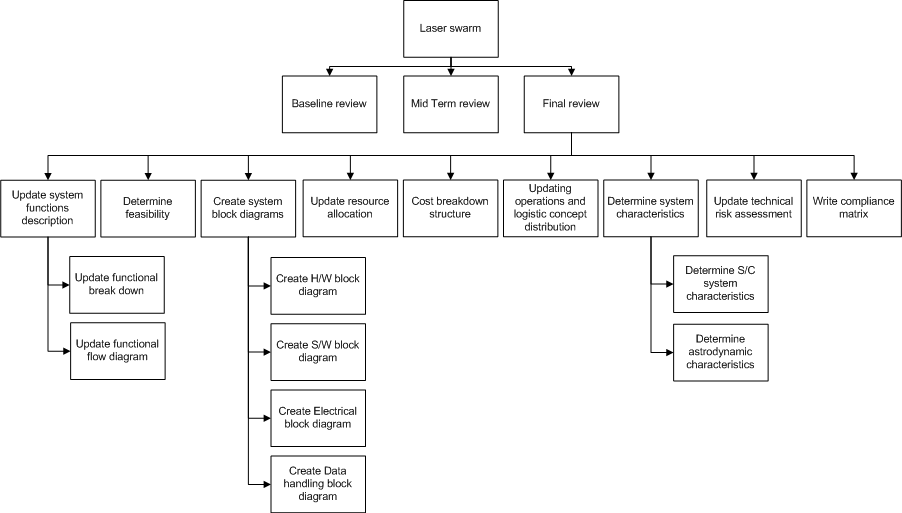
\includegraphics[width=\textheight, angle=90]{chapters/img/Workbreakdown_structure_FR_v2.png}
\caption{Updated work break-down structure for the final report}
\label{fig:WFfinal2}
\end{figure}

\section{Gantt chart}
\label{Gantt}
As the \acp{WFD} and the \acp{WBS} have been updated, so the Gantt chart has also been updated. 
Now that we are further along in the project, it is easier to estimate which tasks need to be done for the mid-term and final reports. The estimated duration of these tasks also was much easier to estimate. The Gantt chart has been updated to contain all tasks set in the \ac{WFD}s. Special care was taken to make sure the Gantt chart is consistent with the \acp{WFD} and the \acp{WBS}.
This time the simulator tasks were not separated from the rest of the project because the simulator is more involved with the 
rest of the project for the mid-term and final reports.
The updated Gantt chart can be found in appendix \ref{ganttChart}, page \pageref{ganttChart}.